\documentclass[tikz,border=8pt]{standalone}
\usepackage{chemfig} % <--- THIS is crucial
\usepackage{tikz}
\usetikzlibrary{arrows.meta,positioning}

\begin{document}
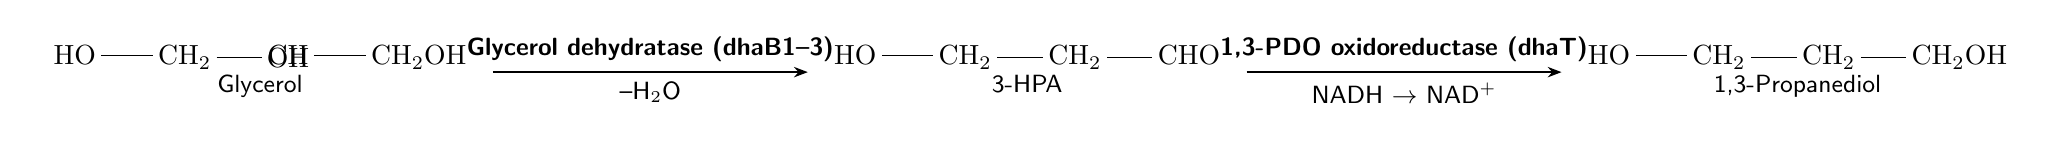
\begin{tikzpicture}[
    arr/.style={-{Stealth[length=5pt]}, thick},
    node distance=4cm,
    font=\sffamily
]

% --- Molecules (simple stick diagrams) ---
\node (glycerol) {
    \begin{tabular}{c}
        \chemfig{HO-CH_2-CH(OH)-CH_2OH}\\[-2pt]
        \small Glycerol
    \end{tabular}
};

\node[right=of glycerol] (hpa) {
    \begin{tabular}{c}
        \chemfig{HO-CH_2-CH_2-CHO}\\[-2pt]
        \small 3-HPA
    \end{tabular}
};

\node[right=of hpa] (pdo) {
    \begin{tabular}{c}
        \chemfig{HO-CH_2-CH_2-CH_2OH}\\[-2pt]
        \small 1,3-Propanediol
    \end{tabular}
};

% --- Arrows ---
\draw[arr] (glycerol) -- (hpa)
    node[midway,above]{\small \textbf{Glycerol dehydratase (dhaB1–3)}}
    node[midway,below]{\small –H$_2$O};

\draw[arr] (hpa) -- (pdo)
    node[midway,above]{\small \textbf{1,3-PDO oxidoreductase (dhaT)}}
    node[midway,below]{\small NADH $\rightarrow$ NAD$^+$};

\end{tikzpicture}
\end{document}
